
\subsection{Intensidad de Corriente}
\begin{wrapfigure}{r}{3cm}
        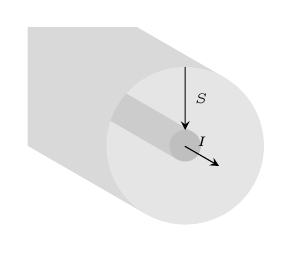
\begin{tikzpicture}
                \clip (-2,-1.1) rectangle (1,1.5);
                \begin{scope}[rotate=-30]
                        \fill[gray!30] (-3,-1) rectangle (0,1);
                        \fill[gray!20] (0,0) circle(1cm);
                        \begin{scope}
                                \clip(0,0) circle(1cm);
                                \fill[gray!40] (-3,-0.2) rectangle (0,0.2);
                                \fill[gray!50] (0,0) circle(2mm);
                        \end{scope}
                        \draw[-stealth] (120:1) -- node[right,font=\tiny]{$S$}(120:0.2);
                        \draw[-stealth] ([yshift=-0.5\pgflinewidth]0,0) -- node[above,font=\tiny]{$I$}([yshift=-0.5\pgflinewidth]0.5,0);
                \end{scope}
        \end{tikzpicture}
\end{wrapfigure}
\noindent Definimos la Intensidad como la cantidad de corriente que circula por una sección de un conductor:
\[
        I \hspace{1mm}= \hspace{1mm} \frac{\mathrm{d}q }{\mathrm{d} t}
\]
\noindent De esta formula podemos también obtener los valores de \(\mathbf{d}\bm{q}\) y por ende \textbf{I}:
\[
        \boxed{\mathrm{d}q \hspace{1mm}= \hspace{1mm} n\hspace{.5mm}\left | q\right |\hspace{.5mm}v_d\hspace{.5mm}S\hspace{.5mm}\mathrm{d}t}
\]
\[
        \boxed{I \hspace{1mm}= \hspace{1mm} n\hspace{.5mm}\left | q\right |\hspace{.5mm}v_d\hspace{.5mm}S\hspace{.5mm}}
\]
Siendo las incógnitas:
\begin{itemize}
        \item \(\bm{n}\): Es el número de cargas que fluyen por unidad de volumen \textbf{C/V}.
        \item \(\bm{v_d}\): Es la velocidad de deriva con que se mueven las cargas \textbf{m/s}.
        \item \(\bm{S}\): Es la sección transversal, su superficie.
        \item \(\bm{q}\): Es el valor de la carga que circula, tomaremos en un principio valores positivos, es decir en valor absoluto.
\end{itemize}
\subsection{Vector Densidad de Corriente}
\noindent Esta es una magnitud vectorial con la cual podemos medir la intensidad que atraviesa una superficie:
\[
        I \hspace{1mm} = \hspace{1mm} \int_{S} \vec{J}\hspace{3mm}\mathrm{d}\hspace{.5mm}\vec{S}\hspace{3mm}\Rightarrow  \boxed{J\hspace{1mm} = \hspace{1mm} \left | \frac{I}{S} \right |}
\]
\subsubsection{Campo Electrostático y Densidad de Corriente}
\noindent Entre \(\bm{\vec{J}}\) y \(\bm{\vec{E}}\) existe una relación muy estrecha, y es que cuanto \(\bm{\vec{E}}\) aumenta, debido a que \(\bm{v_d}\) se incrementa, \(\bm{\vec{J}}\) crece proporcionalmente:
\[
        \bm{\vec{J}} \hspace{2mm} \bm{\alpha} \hspace{2mm} \bm{\vec{E}}
\]
\subsection{Conductores Ohmicos}
\noindent Conocemos ya dos conceptos que nos permitirán deducir la resistividad que posee un material, el \underline{Campo Eléctrostático} y la \underline{Densidad de Corriente}, además de la Ley de Ohm \(\bm{V = IR}\), que relaciona la Tensión con la Resistencia y la Intensidad:
\[
        \vec{J} \hspace{1mm} = \hspace{1mm} \sigma \vec{E}
\]
\[
        \vec{E} \hspace{1mm} = \hspace{1mm} \rho \vec{J}
\]
Siendo \(\bm{\sigma}\) la \underline{Conductividad Eléctrica} en \underline{Siemens} entre metros \textbf{S/m} y \(\bm{\rho}\) la \underline{Resistividad Eléctrica} en ohmios por metro \(\bm{\omega}\)\textbf{m}
\subsubsection{Resistencia}
\noindent Considerando que la caida de tensión entre los extremos de una resistencia vale \\ \(\bm{\Delta V_{\textnormal{ba}}} \hspace{1mm}= \hspace{1mm} \bm{V_\textnormal{b}} -\bm{V_\textnormal{a}}  \Rightarrow \bm{\Delta V_{\textnormal{ba}}}\hspace{1mm}= \hspace{1mm} \bm{E \mathrm{d}l}\) y teniendo en cuenta la definición de \(\bm{\vec{J}}\) podemos concluir en lo siguiente:
\[
        \boxed{\bm{\frac{V}{I} = \frac{E\mathrm{d}l}{\sigma E S} = \frac{\mathrm{d}l}{\sigma S} = \frac{\rho \mathrm{d}l}{S} = R = cte}}
\]
\subsection{Joule}
\noindent Este es un efecto, que se produce en una resistencia, que define que hay una disipación de la energía en forma de calor, ya que al pasar por una resistencia, la tensión que sale \(\bm{V_b}\) es menor que la que entra \(\bm{V_a}\):
\[
        \mathrm{d}Q \hspace{1mm} = \hspace{1mm} cte \hspace{1mm} = \hspace{1mm} I
\]
\[
        \mathrm{d}V \hspace{1mm} = \hspace{1mm} \mathrm{d}Q \Delta V_{\textnormal{ba}}\]
\[
        -\frac{\mathrm{d} v}{\mathrm{d} t} \hspace{1mm} = \hspace{1mm} \frac{\mathrm{d} Q}{\mathrm{d} t}\Delta V_{\textnormal{ab}} \hspace{1mm} = \boxed{P_{\textnormal{disipada}} \hspace{1mm} = \hspace{1mm} V I \textnormal{[\textbf{W}]}}
\]
\subsection{Baterías}
\noindent Las baterías están formadas por un generador interno y una resistencia en serie, este generador produce una f.e.m (\(\bm{\varepsilon}\)). Idealmente:
\[
        W \hspace{1mm} = \hspace{1mm} \Delta U \hspace{1mm} = \hspace{1mm} \Delta QV
\]
\[
        \varepsilon \hspace{1mm} = \hspace{1mm} \frac{W}{\Delta Q} \hspace{1mm} = \hspace{1mm} V
\]
Es decir: \(\boxed{\bm{P_{\textnormal{suministrada}}} \hspace{1mm} = \hspace{1mm} \bm{\varepsilon I - I^2r}}\) en una situación ideal \(\bm{r}=\)0\(\bm{\Omega}\)
\subsection{Leyes de Kirchoff}
\noindent Se aplica a circuitos que no se pueden resolver aplicando las leyes de Ohm solamente, se basa en el uso de mallas que dividen la corriente y su sentido, en función de la orientación de las pilas
\subsubsection{Leyes de los Nudos}
\begin{wrapfigure}{r}{3cm}
        \begin{tikzpicture}
                \draw[->] (-2,0) -- (-1, 0) node[above = 1]{\(\bm{I_1}\)};
                \draw[-] (-1, 0) -- (0, 0);
                \draw[->] (0,0) -- (1,0) node[above = 1]{\(\bm{I_4}\)};
                \draw[->] (0,0) -- (1,-1.2) node[above = 1]{\(\bm{I_2}\)};
                \draw[->] (0,0) -- (1, 1.3) node[above = 1]{\(\bm{I_3}\)};
                \draw[-] (1,0) -- (2,0);
                \draw[-] (1,-1.2) -- (2,-1.2);
                \draw[-] (1, 1.3) -- (2, 1.3);
        \end{tikzpicture}
\end{wrapfigure}
\noindent También conocida como \textbf{LCK}, define como aparece en el esquema que la intensidad que circula por un circuito, es es igual a la suma de todas aquellas intensidades que se generan al pasar por un nodo y bifurcarse. Se define como:
\[
        \boxed{I_T \hspace{1mm} = \hspace{1mm} \sum_{n=1}I_n}
\]
\subsubsection{Leyes de las Mayas}
\noindent También conocida como \textbf{LTK} define que la suma de todas las tensiones de cada malla, debe ser igual a cero:
\[
        \boxed{\sum_{n=1}V_n \hspace{1mm} = \hspace{1mm} 0\textnormal{\textbf{V}}}
\]
\noindent Por defecto consideraremos que si la corriente va del polo positivo al negativo de la pila, tiene sentido negativo, y positivo en el contrario. Esta misma regla se aplicará a las resistencias.
Las resistencias de una misma corriente se sumarán, y en función del sentido de la corriente con la que puedan coincidir, se sumarán si van en el mismo sentido.
\subsubsection{Circuitos simples y Paralelos}
\subsubsection{Simples}
\begin{itemize}
        \item Tensión: La tensión total es la suma de todas las tensiones.
        \item Intensidad: es \textbf{cte}.
        \item Resistencia: La resistencia total es la suma de todas las resistencias.
\end{itemize}
\subsubsection{Paralelos}
\begin{itemize}
        \item Tensión: Es \textbf{cte} porque la carga es la misma en cada rama.
        \item Intensidad: La intensidad total es la suma de todas las intensidades.
        \item Resistencia: La resistencia total es la suma de todas las resistencias, inversas, y nuevamente inversa: \(\bm{\frac{1}{R_T} = \sum_{n = 1}\frac{1}{R_n}}\)
\end{itemize}
\subsection{Transistores}
\begin{wrapfigure}{l}{0cm}
        \begin{tikzpicture}
                \path (0,0) coordinate (ref_gnd);
                \draw
                (ref_gnd)
                to[battery=\(V\)] ++(0,1)
                to[nos] ++(0,2)
                to[R=\(R\)] ++(3,0)
                to[C=\(C\)] ++(0,-3)
                -- (ref_gnd);
        \end{tikzpicture}
\end{wrapfigure}
\noindent El circuito de la figura es un circuito RC, es decir, posee una resistencia y un condensador.
Vamos a estudiar este circuito para dos momentos concretos en el tiempo, en el instante inicial y cuando ha transcurrido mucho tiempo, indefinido.
\vspace{.5cm}
\par \noindent Cuando el circuito se enciende por primera vez, \(\bm{t = 0}\) en el momento en el que se pulsa el interruptor, la intensidad que circula por el circuito es la misma en todo momento, ya que \underline{el condensador está vacio y actua como un cable}.
\vspace{.5cm}
\par \hspace{-0.3cm}Cuando ha pasado un tiempo indefinido \(\bm{\rightarrow \infty}\), deja de circular corriente, porque \underline{el condensador se ha cargado y ahora funciona como un cable roto, hay cortocircuito}.
\\
\\
\noindent Ecuaciones:
\begin{itemize}
        \item \(\bm{Q(t)=Q_f(1-e^{-\frac{t}{RC}})}\)
        \item \(\bm{I(t)=\frac{\varepsilon}{R}e^{-\frac{t}{RC}}}\)
        \item \(\bm{V_R(t) = \varepsilon e^{-\frac{t}{RC}}}\)
        \item \(\bm{V_C(t) = \varepsilon(1-e^{-\frac{t}{RC}})}\)
\end{itemize}
